%%
%% This is file `sample-sigconf.tex',
%% generated with the docstrip utility.
%%
%% The original source files were:
%%
%% samples.dtx  (with options: `sigconf')
%% 
%% IMPORTANT NOTICE:
%% 
%% For the copyright see the source file.
%% 
%% Any modified versions of this file must be renamed
%% with new filenames distinct from sample-sigconf.tex.
%% 
%% For distribution of the original source see the terms
%% for copying and modification in the file samples.dtx.
%% 
%% This generated file may be distributed as long as the
%% original source files, as listed above, are part of the
%% same distribution. (The sources need not necessarily be
%% in the same archive or directory.)
%%
%% The first command in your LaTeX source must be the \documentclass command.
\documentclass[sigconf, nonacm, natbib, screen, balance=False]{acmart}

% Documentation for packages
% - ACM Article Template
%    https://www.acm.org/publications/proceedings-template
% - Pseudocode typesetting CLRS-style:
%    https://www.cs.dartmouth.edu/~thc/clrscode/clrscode3e.pdf
% - Python code typesetting
%    http://ctan.uib.no/macros/latex/contrib/listings/listings.pdf
% - AMS Math
%    http://ctan.uib.no/macros/latex/required/amsmath/amsldoc.pdf
% - Graphics
%    http://ctan.uib.no/macros/latex/required/graphics/grfguide.pdf

\usepackage{clrscode3e}  
\usepackage{listings}
\usepackage{cite}
\usepackage{placeins}
\lstset{language=Python, basicstyle=\ttfamily}

% based on https://tex.stackexchange.com/questions/279240/float-for-lstlisting
\usepackage{float}
\floatstyle{ruled}
\newfloat{listing}{tbph}{lop}
\floatname{listing}{Listing}
\def\lstfloatautorefname{Listing} % needed for hyperref/auroref

\citestyle{acmauthoryear}

%% end of the preamble, start of the body of the document source.
\begin{document}

%%
%% The "title" command has an optional parameter,
%% allowing the author to define a "short title" to be used in page headers.
\title{Runtime analysis of sorting algorithms}
\subtitle{INF221 Term Paper, NMBU, Autumn 2020}

\author{Eirik Høyheim}
\email{eirik.hoyheim@nmbu.no}
\affiliation{}  % separates Jane's and Joe's author block

\author{Sebastian Becker}
\email{sebabeck@nmbu.no}

%% The abstract is a short summary of the work to be presented in the
%% article.
\begin{abstract}
There exists extensive research about the theoretical runtime of various sorting algorithms. In this paper we investigate real-life behaviour of quadratic algorithms (Insertion sort and Bubble sort), sub-quadratic algorithms (Mergesort and Quicksort) and the combined algorithm Timsort. We will also look at Pythons built-in sorting functions NumPy sort and Python sort. The algorithms are implemented in Python and tested by sorting various list types of various sizes. List types we use are increasing list, decreasing list, random integer list, random float list and string list. The main result in this paper was that quadratic algorithms had the longest runtime for sorting lists, with exception of list sizes between 10-40, where they outperform the sub-quadratic algorithms. The built-in sorting functions outperformed the other algorithms in every test case. Conclusion of this paper is that all algorithms tested in this experiment has the same real-life behaviour as the theoretical performance, except Timsort on increasing lists.  

\end{abstract}


%%
%% This command processes the author and affiliation and title
%% information and builds the first part of the formatted document.
\maketitle

\section{Introduction}\label{sec:intro}

Theoretical analysis of sorting algorithms is a common subject taught at universities for computer science. Sorting algorithms is an important field in computer science. Advantages of using the optimal algorithm in a specified case can be the difference between success and failure. Therefore, we consider the topic discussed in this paper as an important field to investigate. The algorithms we will investigate in this paper are Insertion sort, Bubble sort, Quicksort, Mergesort, Timsort and the built-in sorting functions NumPy sort and Python sort. 

Our motivation in this paper is to learn more about how different sorting algorithms preform in real-life behaviour. In this paper we examine: is it possible to obtain the theoretical runtime of different sorting algorithms in real-life applications? We will also investigate whether some of the sorting algorithms in this paper have any advantages or disadvantages.

This paper starts with a brief description of the necessary theoretical background. Then, we will explain why and how we conducted the experiment. After this we will describe the main results. At the end we will discuss our results and present further investigations. 

\section{Theory}\label{sec:theory}
The main source in this section is the book Introduction to Algorithms. For more information about the book, look at references. Bubble sort and Timsort are not deeply described in the book, therefore we have used other sources for those. 


\subsection{Insertion sort}\label{sec:algo1}
Pseudocode for Insertion sort is shown in Listing~\ref{lst:insertion_algo}. Insertion sort starts with a sorted part A[1...j-1] and an unsorted part A[j... A.length]. The j-th element of the unsorted part gets compared with elements in the sorted part and is placed to the right of the element with smaller or equal value of itself. The algorithm terminates when all elements from the unsorted part is placed in the sorted part. Insertion sort is a stable algorithm, because the order of elements with same value will be the same for the input list as in the output list. \citet{CLRS_2009} 

Insertion sort has a space complexity of O(1). This is because only the element to be placed correctly in the sorted part occupies extra memory. \citet{insertion_sort}

Best-case runtime for Insertion sort is achieved when the data is monotonically increasing. The runtime is then proportional to the size of the data. Time complexity is then 
\begin{equation*}
T(n) = \Theta(n). 
\end{equation*}
$T(n)$ is the runtime of a problem where $n$ represent the size of the input list. $\Theta$ is the asymptotically upper and lower bound. 
Worst-case runtime is achieved when input data is monotonically decreasing. The runtime is then 
\begin{equation*}
T(n) = \Theta(n^2).
\end{equation*}
Expected runtime for monotonically increasing list will increase linearly for larger input lists. For monotonically decreasing we can expect a quadratic increase of runtime for larger input lists. Average runtime is expected to be $\Theta(n^2)$. \citet{CLRS_2009}
 
\begin{listing}
  % Pseudocode caption above the code.
  \caption{Insertion sort algorithm from \citet[Ch.~2.1]{CLRS_2009}.}
  \label{lst:insertion_algo}
  %
  % For documentation on how to typeset CLRS-style pseudocode, see
  % https://www.cs.dartmouth.edu/~thc/clrscode/clrscode3e.pdf
  %
  \begin{codebox}
    \Procname{$\proc{Insertion-Sort}(A)$}
    \li \For $j \gets 2$ \To $\attrib{A}{length}$
    \li \Do
    $\id{key} \gets A[j]$
    \li // insert A[j] into the sorted sequence A[1..j-1].
    \li     $i \gets j-1$
    \li      \While $i>0$ and $A[i] > \id{key}$
    \li      \Do
    $A[i+1] \gets A[i]$
    \li         $i \gets i-1$
    \End    
    \li       $A[i+1]\gets \id{key}$
    \End
  \end{codebox}
\end{listing}
\FloatBarrier




\subsection{Bubble sort }\label{sec:algo2}
Pseudocode for Bubble sort is shown in Listing~\ref{lst:bubble_algo}. Bubble sort iterates through the input list and compare pairwise elements next to each other. It switches place between the elements when A[j-1] is bigger than A[j]. The iteration will continue until the largest value in the list is at the end of the list. Bubble sort will continue with this procedure until all elements are sorted in increasing order. \citet{bubble_sort}

Bubble sort is a stable algorithm. Space complexity of Bubble sort is O(1). Expected runtime for all scenarios is 
\begin{equation*}
T(n)=\Theta(n^2).
\end{equation*}
Runtime is expected to increase quadratically as input list increases. \citet{bubble_sort}

We can optimize Bubble sort by implementing a boolean flag which checks if any elements have changed place. If no elements have changed place, then the list is already sorted. Therefore, no reason to loop further through the list. With respect to runtime, the best-case for the optimized Bubble sort is when the input list is increasing. Worst-case occurs when the input list is decreasing. Expected best-case runtime for the optimized Bubble sort will increase linearly as input list increases. Worst-case runtime is expected to increase quadratic as input list increases. Average runtime for the optimized Bubble sort will increase quadratic as input list increases.
\begin{equation*}
 \text{Best case optimized: } T(n) = \Theta(n). 
\end{equation*}
\begin{equation*}
 \text{Worst case optimized: } T(n) = \Theta(n^2). 
\end{equation*}
\begin{equation*}
 \text{Average case optimized: } T(n) = \Theta(n^2). 
\end{equation*}
\citet{bubble_sort}
	\begin{listing}
	  % Pseudocode caption above the code.
	  \caption{Bubble sort algorithm \citet[Ch.~2]{CLRS_2009} }
	  \label{lst:bubble_algo}
	  %
	  % For documentation on how to typeset CLRS-style pseudocode, see
	  % https://www.cs.dartmouth.edu/~thc/clrscode/clrscode3e.pdf
	  %
	  \begin{codebox}
	    \Procname{$\proc{Bubble-Sort}(A)$}
	    \li \For $i \gets 2$ \To $\attrib{A}{length}-1$
	    \Do
	    \li \For $j \gets 2$ \To $\attrib{A}{length}-i+1$
	    \Do
	    \li \If $ A[j] < A[j-1]$
	    \Do
	    \li exhange $A[j]$ with $A[j-1]$
	    \End
	    \End
	  \end{codebox}
	\end{listing}
\FloatBarrier
\subsection{Mergesort }\label{sec:algo3}

    \begin{listing}
	  % Pseudocode caption above the code.
	  \caption{Mergesort algorithm from \citet[Ch.~2.3]{CLRS_2009}.}
	  \label{lst:merge_algo}
	  %
	  % For documentation on how to typeset CLRS-style pseudocode, see
	  % https://www.cs.dartmouth.edu/~thc/clrscode/clrscode3e.pdf
	  %
	  \begin{codebox}
	    \Procname{$\proc{Merge-Sort}(A, p, r)$}
	     \li \If $p<r$
		\Do
		\li $q \gets \lfloor(2p+r)/2\rfloor$
		\li $\proc{Merge-Sort}(A,p,q)$
		\li $\proc{Merge-Sort}(A,q+1,r)$
		\li $\proc{Merge}(A,p,q,r)$
		\End
	  \end{codebox}
	  \begin{codebox}
		\Procname{$\proc{Merge}(A,p,q,r)$}
		\li $n_1 \gets q-p+1$
		\li $n_2 \gets r-q$
		\li \For $ i=1 \text{ to } n_1$
		\Do
		\li $L[i] \gets A[p+i-1]$
		\End
		\li \For $j \gets 1 \text{ to } n_2$
		\Do
		\li $R[j] \gets A[q+j]$
		\End
		\li $L[n_1+1]\gets \infty$
		\li $R[n_2+1]\gets \infty$
		\li $i=1$
		\li $j=1$
		\li \For $k=p \text{ to } r$
		\Do
		\li \If $L[i] \leq R[j]$
		\Do
		\li $A[k] = L[i]$
		\li $i = i+1$
		\li \Else $A[k]=R[j]$
		\li $j=j+1$
		\End
		\End
	  \end{codebox}
	\end{listing}
\FloatBarrier
Pseudocode for Mergesort is shown in Listing~\ref{lst:merge_algo}. Mergesort follows the divide and conquer approach. Divide and conquer approach follow three steps. First step it divides the problem into smaller subproblems. In the second step it solves these subproblems by using recursion. The last step it combines the solutions of these subproblems into the solution for the original problem. \citet{CLRS_2009}.

Mergesort has the same expected runtime for various list types of various sizes. Since Mergesort follows the divide and conquer approach, it will always divide the input list into two halves until it has subproblems that contains one element. Then the merge process starts and combines the subproblems into a sorted sequence. The merge process continues until all the sequences is merged into a completely sorted list. Expected runtime for Mergesort will be     

\begin{equation*}
	T(n) = \Theta(n\lg(n)).
\end{equation*} 
\citet{CLRS_2009} 

\subsection{Quicksort }\label{sec:algo4}
\begin{listing}
	  % Pseudocode caption above the code.
	  \caption{Quicksort algorithm from \citet[Ch.~7.1]{CLRS_2009}.}
	  \label{lst:quick_algo}
	  %
	  % For documentation on how to typeset CLRS-style pseudocode, see
	  % https://www.cs.dartmouth.edu/~thc/clrscode/clrscode3e.pdf
	  %
	  \begin{codebox}
	    \Procname{$\proc{Quicksort}(A, p, r)$}
	     \li \If $p<r$
		\Do
		\li$q \gets \proc{Partition}(A,p,r)$
		\li $\proc{Quicksort}(A,p,q-1)$
		\li $\proc{Quicksort}(A,q+1,r)$
		\End
	  \end{codebox}
	  \begin{codebox}
		\Procname{$\proc{Partition}(A,p,q,r)$}
		\li $x \gets A[r]$
		\li $i \gets p-1$
		\li \For $ j= p \textbf{ to } r-1$
		\Do
		\li \If $A[j] \leq x$
		\Do
		\li $i = i+1$
		\li exchange A[i] with A[j]
		\End
		\End
		\li exchange $A[i+1]$ with $A[r]$
		\li \textbf{return} i + 1
	  \end{codebox}
\end{listing}
\FloatBarrier
Pseudocode for Quicksort is shown in Listing~\ref{lst:quick_algo}. Quicksort uses the divide and conquer approach. First step is to pick the last element in the input list as pivot. Then rearrange the input list into two sublists. Each element in the left sublist must be less or equal to the pivot, and each element in the right sublist must be greater or equal to the pivot. Next step is to sort the two sublists by recursively calling Quicksort. Last step is to combine the sorted sublists to create the sorted list. \citet{CLRS_2009}.

Runtime for Quicksort is dependent on the number of partitions. Best-case is obtained when all partition divides the list into two sublists with size of $n/2$. Expected best-case runtime is then
\begin{equation*}
T(n) = \Theta(n\lg(n)).
\end{equation*} 
Worst-case behaviour for Quicksort occurs when all partitions return two sublists, where one sublist contains n -1 elements and the other sublist contain 0 elements. Expected worst-case runtime is then
\begin{equation*}
T(n)=\Theta(n^2).
\end{equation*}
\citet{CLRS_2009}

Randomized Quicksort is an optimized version of Quicksort. It use randomized partitions to avoid worst-case. Expected runtime of the optimized Quicksort is 
\begin{equation*}
T(n) = \Theta(n\lg(n)).
\end{equation*} 
\citet{CLRS_2009}

\subsection{Timsort }\label{sec:algo5}

The main source for this paragraph is \citet{kumar_2020}, marked if another source is used. Timsort is a sorting algorithm that combines Insertion sort and Mergesort. Timsort divides the input data in small sublists. These sublists get sorted individually by using Insertion sort. The size of a sublist can vary, but it has a minimum size that the Timsort algorithm calculates for us. Mergesort combines the sorted sublists into one sorted list. Timsort is a stable algorithm, with an expected best-case runtime 

\begin{equation*}
T(n) = \Theta(n) 
\end{equation*}
and an expected worst-case runtime
\begin{equation*}
T(n) = \Theta(n\lg(n)).
\end{equation*}
Equations collected from \citet{tim-sort}.

\section{Methods}\label{sec:methods}
In this section we are going to describe how we conducted our experiment and why we did it this way.
\subsection{Algorithms}

In this paper we look at five different sorting algorithms, Insertion sort, Bubble sort, Mergesort, Quicksort and Timsort. The built-in sorting functions Python sort and NumPy sort is also a part of this paper to compare how they preform against the algorithms. We look at how fast the algorithms preform against lists of different types and sizes. All the algorithms are in different files. We benchmark one algorithm at a time to prevent overworking the computer and effecting results. When running a benchmark, we try to make the computer only work on the benchmark process by not having any unnecessary programs running in the background.

\subsection{Generating lists}

The different list types we use to measure the performance of the different algorithms are increasing list, decreasing list, string list, random float list and random integer list. Reason for choosing these list types, is to examine the behaviour of the different algorithms under specified situations. A majority of algorithms in this paper have their best and worst performance when the input data is increasing and decreasing, respectively. Therefore, we find it convenient to implement decreasing list and increasing list. In addition, we want to investigate if some of the algorithms have an advantage or a disadvantage when sorting specified, random list types. Random integer list, random float list and string list give an overall view on how algorithms can perform when we do not know anything about the given list. It will also represent average case. 

Our five, independent list functions take size as input, where size indicates the length of the list that we create. These functions return the specified list type with the specified size. Reason for taking size as input is to automate our benchmark process by making it easier to create lists with different sizes. We create random float list and random integer list with NumPy’s random list generator. For creating increasing list, we use pythons built-in function, $list(range(size))$. Decreasing list is made by reversing an increasing list. We create string list by making an array containing all letters in the English alphabet and then randomly picking letters from the array. 

We have implemented test-cases which all list types must pass. This is done to avoid implementation something illogical. Test for the lists is in $test\_list\_builders.py$, and Git hash can be found in Table \ref{tab:hashes}.

\subsection{Benchmark and runtime}

Benchmarks are calculated using $time\_algorithm$ function given in Table \ref{tab:hashes}. All the list types with different size are used to measure the performance of each algorithm. We assured, that lists of same type and size are identical for all algorithms by adding a seed in the beginning of $time\_algorithm$ function, as shown in Listing \ref{lst:bench_setup}. Problem with seed is that some random lists may be partly sorted by chance. Since we test the algorithms with different list types of various sizes, it will probably cover such errors. 

The $time\_algorithm$ function will automatically go through all list types, one at a time, for the algorithm that is chosen. Our benchmark function will first create a list type at list length 10, and then begin the benchmarking process. When the benchmark result has been produced, we will increase the next list size by taking the previous list size and multiplying it by 2. This will give list number $t$ a size of 10 $\cdot$ $2^{t-1}$. This process will happen until expected runtime $t\_ar$ will pass 5 seconds for one iteration, which is shown in Listing \ref{lst:bench_setup}.

To ensure that we do not just sort the first list, we copy the list every time we run the benchmark process. After every list type has gone through the nested iteration, we store the minimum time taken in each result in a dictionary. We do this to show the best possible time, out of five rounds in the benchmark process. Python function $timeit.repeat$, which we used to measure time, documentation, \citet{timeit}, recommended to only store the minimum value. 
The results are stored, using pandas $to\_pickle$ function, with three columns: list type, list size and time. The variable containing the result is named after the algorithm.

Since the same list with the same list size is equal for all algorithms, we can easier see how different list types effects different algorithms. When plotting, we split up the data from the different algorithms and distinguish between list types, because we want to see how different algorithms handle different situations. Our figures are made without error bars. When plotting all five results from one iteration, we got an error bar that was smaller than symbol size. Consequently, we chose to only include the fastest time from each iteration instead of all points, because \citet{timeit} recommended to do so. We use a log-10 scale in x and y direction on all figures because of large variance between list sizes and runtime in our results. This will also make symbols more visible. The downside of doing this is that it is not always clear how algorithms preform at smaller list sizes, such as lists with size between 0 and 1000. 

Consequently, we will add tables to distinguish between smaller list sizes. This will also make it easier to see any special trend for each algorithm and compare these with one another. The tables are made using $to\_latex()$ and show list sizes from 0 to 10’240. In each row, there is one bold number. This number is the fastest algorithm at the given list size. Although probably Python sort and NumPy sort are faster than all the other algorithms, we chose not to mark any of their results, because we wanted to see which non built-in algorithm was the fastest.

It is essential that we know that all algorithms sort in increasing order, or else we will get unreliable results. Therefore, we implemented tests, and made sure that all algorithm passed with all the different list types, before running benchmarks. The test to check that all algorithms sort in increasing order is in $test\_sort\_algos.py$, and Git hash can be found in Table \ref{tab:hashes}


\begin{listing}[h!]
  % Listing captions above the listing.   
  \caption{Benchmark setup. For full bechmark setup, see githash in Table \ref{tab:hashes}}
  \label{lst:bench_setup}
  \begin{lstlisting}
np.random.seed(seed)
for new_list in lists:
     t_ar = 0
     size = 10
     while t_ar < 5:
         try:
             data = new_list(size)

		...

	     size  = 2*size
  \end{lstlisting}
\end{listing}
\FloatBarrier


\begin{table}[h!]
  % Table captions always come *above* the table.
  \caption{Versions of files used for this report; GitLab repository
    \url{https://gitlab.com/nmbu.no/emner/inf221/h2020/student-term-papers/team_10/inf221-term-paper-team10.git}.}
  \label{tab:hashes}
  \begin{tabular}{ll}
    \hline
    File & Git hash \\\hline
    \verb!test_list_builders.py! & \verb!a4c92d29! \\
    \verb!test_sort_algos.py! & \verb!cd78ea21! \\
    \verb!time_algorithm.py! & \verb!877f68a6! \\
    \verb!tables_random_lists.ipynb! & \verb!5035bdcb! \\
    \verb!tables_sorted_lists.ipynb! & \verb!5035bdcb! \\
  \end{tabular}
\end{table}
\FloatBarrier

\section{Results}\label{sec:results}

In this section we present our benchmark results. When stating that algorithms are increasing quadratically, we mean that the runtime is increasing with approximately a factor of 4 when list size is doubled. By increasing linearly, we mean that the runtime is increasing with approximately a factor of 2 when list size is doubled.
All results can be found in $tables\_random\_lists.ipynb$ and $\\tables\_sorted\_lists.ipynb$, Git hash given in Table \ref{tab:hashes}. Here you can find tables for random lists and sorted lists, respectively. 

\subsection{Random integer list}

There are three main groups in relation to runtime in Figure \ref{fig:rand_int}. We observe that the algorithms in the same groups have similar runtime. Group one consists of the quadratic algorithms, which are the slowest sorting algorithms. The next group contains the sub-quadratic algorithms and Timsort. Group three is the built-in sorting functions, which have the shortest runtime. We can see from Figure \ref{fig:rand_int} that Python sort is faster than NumPy sort when list size is smaller than $10^2$. For list sizes larger than $10^2$, NumPy sort is faster than Python sort.


\begin{figure}[h!]
  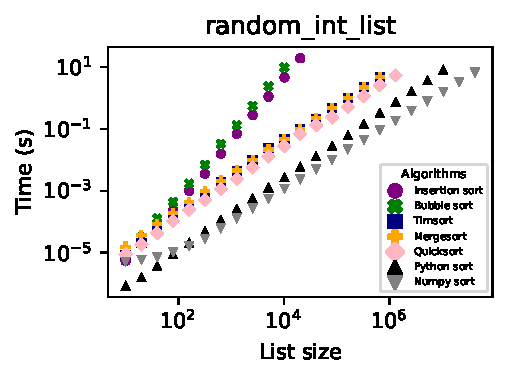
\includegraphics[width=\linewidth]{../figures/random_int_list.pdf}
  \caption{Benchmark results for random integer lists. Time (s) is in seconds and Size (n) is number of elements. Scale is log-10 in both n [horisontal] and s [vertical] directions.}
  \label{fig:rand_int}
\end{figure}
\FloatBarrier


In Table \ref{tab:integer} we see a snippet of runtime for the different algorithms running on random integer list. We observe that quadratic algorithms have better or equal runtime as the sub-quadratic algorithms and Timsort when list size is between 10-40. Insertion sort use on average approximately half the time of Bubble sort when sorting random integer lists. Runtime for the quadratic algorithms increases quadratically for bigger input list. Further, we observe that Quicksort is the fastest algorithm, besides NumPy sort and Python sort. Quicksort is almost twice as fast as Mergesort and Timsort.

\begin{table}[h!]
\caption{Table with benchmark results for random integer list, data in microseconds. Bold number fastest time at given row, not looking at NumPy- and Python sort}
\label{tab:integer}
\scalebox{0.7}{
\begin{tabular}{lrrrrrrr}

\toprule
Algorithm &  Bubble &  Insertion &  Merge &  Numpy &  Pyhton &  Quick &    Tim \\
size     &              &                 &             &             &              &             &             \\
\midrule
10       &        7.71  &             \textbf{5.44}  &       15.81 &        5.02 &         0.87 &        9.08 &        8.56 \\
20       &        31.29 &           18.58 &       37.14 &        5.83 &         1.64 &        \textbf{18.33} &       21.00 \\
40       &       127.63 &           57.21 &       86.53 &        7.30 &         3.89 &        \textbf{42.76} &       54.71 \\
80       &       437.71 &          239.02 &      187.13 &       10.44 &         9.04 &      \textbf{106.33} &      139.03 \\
160      &      1712.26 &         1006.80 &      433.69 &       16.28 &        21.48 &       \textbf{248.35} &      332.41 \\
320      &      6883.41 &         3576.36 &      974.05 &       28.34 &        50.88 &       \textbf{512.90} &      807.99 \\
640      &     32826.15 &        15901.00 &     2143.39 &       61.06 &       115.81 &      \textbf{1140.16} &     1919.34 \\
1280     &    132777.27 &        70110.37 &     4553.60 &      126.92 &       263.36 &      \textbf{2431.64} &     4335.89 \\
2560     &    556930.00 &       280568.27 &    10062.85 &      269.67 &       584.12 &      \textbf{5716.58} &    10054.66 \\
5120     &   2370172.00 &      1108111.10 &    21737.05 &      558.43 &      1286.85 &     \textbf{12889.39} &    23768.62 \\
10240    &   9637399.60 &      4624960.50 &    47294.56 &     1148.95 &      2810.41 &    \textbf{ 27867.25} &    46967.00 \\
\bottomrule
\end{tabular}
}
\end{table}
\FloatBarrier


\subsection{Random float list}

We observe that Figure \ref{fig:random float} is almost identical with Figure \ref{fig:rand_int}. This implies that algorithms tested in this paper have similar runtime for sorting random float lists and random integer lists. We observe that the quadratic algorithms still have the slowest runtime. Built-in sorting functions have still the fastest runtime, the sub-quadratic algorithms and Timsort lies between these two groups. In relation to the size of the lists we have the same results, despite Mergesort runs one extra iteration on random float list.


\begin{figure}[h!]
  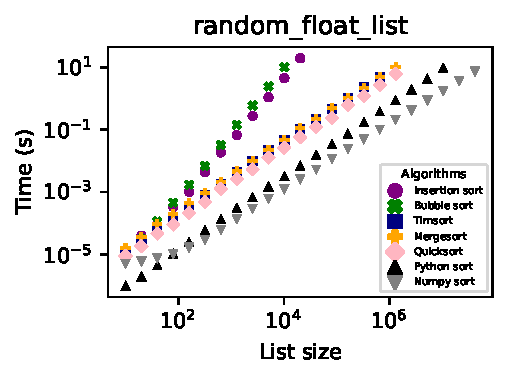
\includegraphics[width=\linewidth]{../figures/random_float_list.pdf}
  \caption{Benchmark results for random float lists. Time (s) is in seconds and Size (n) is number of elements. Scale is log-10 in both n [horisontal] and s [vertical] directions.}
  \label{fig:random float}
\end{figure}
\FloatBarrier


\subsection{Random string list}

Figure \ref{fig:random string} differs from Figure \ref{fig:rand_int} and \ref{fig:random float}, but there are still some similarities. Quadratic algorithms have still the slowest runtime and the built-in sorting functions have still the fastest runtime. The difference lies in the sub-quadratic algorithms. Mergesort and Timsort have similar result as in Figure \ref{fig:rand_int} and \ref{fig:random float}. Quicksort has one major change for list size larger than $10^3$, we now observe that Quicksort gets sufficiently slower than Timsort and Mergesort. In relation to the gap between runtime of Quicksort and Timsort and Mergesort, the runtime difference increases along with larger list sizes. There is also a change in the built-in sorting functions. In Figure \ref{fig:random string}, NumPy sort is quicker than Python sort after lists larger than $10^3$, where in Figure \ref{fig:rand_int} and \ref{fig:random float} this value is at $10^2$. We observe that the difference in runtime between NumPy sort and Python sort is smaller in Figure \ref{fig:random string} than in Figure \ref{fig:rand_int} and \ref{fig:random float}. 

\begin{figure}[h!]
  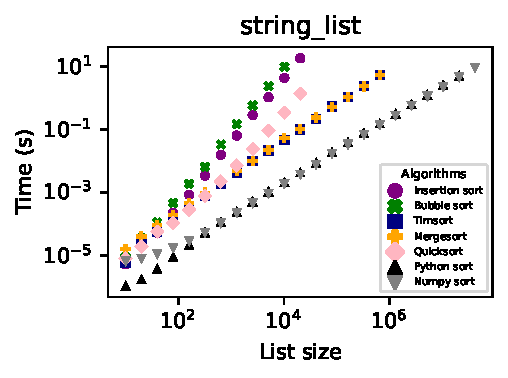
\includegraphics[width=\linewidth]{../figures/string_list.pdf}
  \caption{Benchmark results for random string lists. Time (s) is in seconds and Size (n) is number of elements. Scale is log-10 in both n [horisontal] and s [vertical] directions.}
  \label{fig:random string}
\end{figure}
\FloatBarrier

From Table \ref{fig:string_table} we observe that Quicksort is no longer the fastest sorting algorithm in every case as in random integer lists and random float lists. We also observe that for list size larger than 640, Quicksort gets slower than Timsort and Mergesort. For even larger lists sizes the difference in runtime increases between Quicksort and Timsort and Mergesort. For list sizes of 40 and smaller, Insertion sort is faster than the sub-quadratic algorithms and Timsort.

\begin{table}[h!]
  \caption{Table with benchmark results for string list, data in microseconds. Bold number fastest time at given row, not looking at NumPy- and Python sort}
  \label{fig:string_table}
\scalebox{0.7}{
\begin{tabular}{lrrrrrrr}
\toprule
Algorithm &  Bubble &  Insertion &    Merge &   Numpy &  Pyhton &   Quick &     Tim \\
size     &              &                 &               &              &              &              &              \\
\midrule
10       &         8.58 &            \textbf{5.18} &       15.56 &        6.39 &         1.08 &        7.84 &        5.78 \\
20       &        34.22 &           \textbf{18.64} &       39.17 &        7.74 &         1.74 &       18.98 &       25.15 \\
40       &       110.89 &           \textbf{51.73} &       91.79 &       10.56 &         3.81 &       56.18 &       54.84 \\
80       &       457.79 &          222.25 &      193.89 &       16.56 &         8.95 &      \textbf{104.22} &      139.09 \\
160      &      1843.56 &          835.11 &      440.39 &       27.42 &        21.71 &      \textbf{281.66} &      322.80 \\
320      &      6426.35 &         3383.83 &      974.07 &       50.56 &        52.30 &      \textbf{755.23} &      765.87 \\
640      &     32747.48 &        15353.03 &     2103.81 &      102.00 &       114.25 &     2183.64 &     \textbf{1853.72} \\
1280     &    143920.70 &        62730.10 &     4712.57 &      215.55 &       246.54 &     7022.39 &     \textbf{4223.77} \\
2560     &    566998.90 &       280347.45 &     9826.05 &      440.97 &       511.92 &    23515.70 &     \textbf{9547.42} \\
5120     &   2320593.70 &      1031584.30 &    21986.50 &      890.77 &      1048.46 &    89386.64 &    \textbf{20849.81} \\
10240    &   9623402.30 &      4237909.70 &    52047.02 &     1782.83 &      2121.67 &   332108.55 &    \textbf{45948.43} \\
\bottomrule
\end{tabular}}
\end{table}
\FloatBarrier 


\subsection{Increasing list}

Except Python sort and NumPy sort, Insertion sort is the fastest sorting algorithm on increasing lists, as we see in Figure \ref{fig:increasing}. Timsort and Insertion sort has similar runtime for list sizes of 20 and smaller. For list size larger than 20, Timsort makes a jump in runtime and has similar runtime as Mergesort. For list size 20 and smaller, Insertion sort and Timsort has faster runtime than NumPy sort. Furthermore, we can see from Figure \ref{fig:increasing} that Quicksort is slower than Mergesort and Timsort. Quicksort and Bubble sort has now approximately the same runtime. Python sort has the fastest runtime for all list sizes.     

\begin{figure}[h!]
  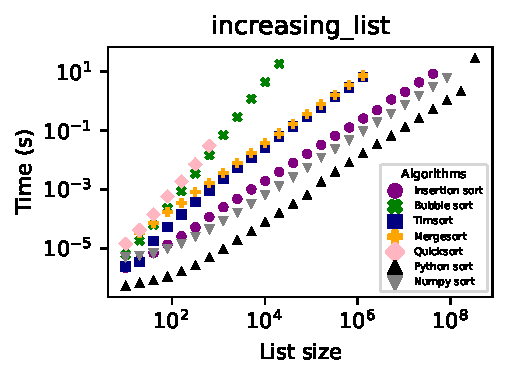
\includegraphics[width=\linewidth]{../figures/increasing_list.pdf}
  \caption{Benchmark results for increasing lists. Time (s) is in seconds and Size (n) is number of elements. Scale is log-10 in both n [horisontal] and s [vertical] directions.}
  \label{fig:increasing}
\end{figure}
\FloatBarrier

From the Table \ref{tab:increasing_table} we see that Insertion sort has almost a linear increment in runtime for larger list sizes. Bubble sort and Quicksort have approximately a quadratic increment in runtime for larger list sizes. We can also see that Timsort do not follow a linear increase of runtime for list sizes between 20 and 40, where it makes a jump. For increasing list, NumPy sort is slower than both Insertion sort and Timsort when list size is smaller than 80.

\begin{table}[h!]
  \caption{Table with benchmark results for inreasing list, data in microseconds. Bold number fastest time at given row, not looking at NumPy- and Python sort}
  \label{tab:increasing_table}
\scalebox{0.7}{
\begin{tabular}{lrrrrrrr}
\toprule
Algorithm &   Bubble &  Insertion &   Merge &   Numpy &   Pyhton &  Quick &     Tim \\
size      &               &                 &              &              &               &             &              \\
\midrule
10        &         6.17 &            \textbf{2.17} &       14.61 &        4.89 &         0.54 &       14.16 &        2.40 \\
20        &        18.44 &            3.93 &       33.79 &        5.54 &         0.68 &       42.05 &        \textbf{3.47} \\
40        &        63.44 &            \textbf{6.96} &       71.64 &        6.72 &         0.82 &      145.04 &       17.73 \\
80        &       230.99 &           \textbf{13.24} &      167.99 &        9.34 &         1.12 &      589.76 &       53.50 \\
160       &       877.26 &           \textbf{25.70} &      348.58 &       14.07 &         1.68 &     1862.24 &      141.53 \\
320       &      3494.50 &           \textbf{52.06} &      830.83 &       23.91 &         2.76 &     7247.75 &      379.32 \\
640       &     14481.11 &          \textbf{115.73} &     1661.68 &       43.50 &         5.08 &    29992.09 &      922.58 \\
1280      &     69735.80 &          \textbf{247.24} &     3699.15 &       82.82 &         9.72 &         NaN &     2266.53 \\
2560      &    287588.00 &          \textbf{477.89} &     7993.77 &      160.87 &        19.39 &         NaN &     5270.02 \\
5120      &   1193686.30 &         \textbf{1005.31} &    17457.36 &      318.09 &        38.95 &         NaN &    11979.83 \\
10240     &   4412479.10 &         \textbf{1938.84} &    37269.94 &      636.06 &        79.25 &         NaN &    26589.77 \\
\bottomrule
\end{tabular}}
\end{table}
\FloatBarrier 


\subsection{Decreasing list}

We observe that there is a big difference in Figure \ref{fig:increasing} and \ref{fig:decreasing_list}. Insertion sort, Bubble sort and Quicksort are the slowest algorithms in the decreasing case. Mergesort is slightly faster than Timsort. Python sort is the fastest algorithm for sorting decreasing lists for all list sizes. 
\begin{figure}[h!]
  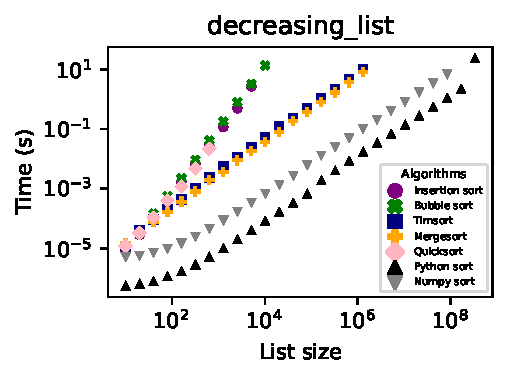
\includegraphics[width=\linewidth]{../figures/decreasing_list.pdf}
  \caption{Benchmark results for decreasing lists. Time (s) is in seconds and Size (n) is number of elements. Scale is log-10 in both n [horisontal] and s [vertical] directions.}
  \label{fig:decreasing_list}
\end{figure}
\FloatBarrier

We see from Table \ref{tab:decreasing_table} that Insertion sort, Bubble sort and Quicksort have approximately a quadratic increment in runtime for larger list sizes. Insertion sort is the fastest sorting algorithm of the quadratic and sub-quadratic algorithms for a list size up to 20. 

\begin{table}[h!]
  \caption{Table with benchmark results for decreasing list, data in microseconds. Bold number fastest time at given row, not looking at NumPy- and Python sort.}
  \label{tab:decreasing_table}
\scalebox{0.7}{
\begin{tabular}{lrrrrrrr}
\toprule
Algorithm &   Bubble &  Insertion &   Merge &   Numpy &   Pyhton &  Quick &      Tim \\
size      &               &                 &              &              &               &             &               \\
\midrule
10        &        11.58 &            \textbf{8.14} &       15.04 &        5.02 &         0.56 &       12.07 &        12.04 \\
20        &        40.54 &           \textbf{28.15} &       35.74 &        5.59 &         0.66 &       32.93 &        41.12 \\
40        &       147.17 &          108.33 &       \textbf{76.03} &        6.83 &         0.81 &      107.24 &        92.87 \\
80        &       575.29 &          400.18 &      \textbf{165.06} &        9.43 &         1.17 &      401.15 &       208.71 \\
160       &      2243.52 &         1695.51 &      \textbf{371.73} &       14.55 &         1.77 &     1200.84 &       439.31 \\
320       &      9317.49 &         6776.09 &      \textbf{807.78} &       24.71 &         2.91 &     4766.62 &      1075.64 \\
640       &     41476.50 &        26980.01 &     \textbf{1934.93} &       45.25 &         5.29 &    21556.60 &      2362.90 \\
1280      &    179954.80 &       116043.28 &     \textbf{3736.94} &       85.88 &        10.31 &         NaN &      5512.59 \\
2560      &    807184.10 &       494264.65 &     \textbf{8938.38} &      168.93 &        20.37 &         NaN &     11827.50 \\
5120      &   3291701.30 &      2681181.60 &    \textbf{18603.21} &      336.38 &        40.72 &         NaN &     25213.85 \\
10240     &  13447597.70 &             NaN &    \textbf{37616.11} &      673.26 &        83.91 &         NaN &     53530.22 \\
\bottomrule
\end{tabular}
}
\end{table}
\FloatBarrier 


\section{Discussion}\label{sec:discussion}
In this section we will discuss our result, found in section \ref{sec:results}.
When talking about random lists we mean random integer list, random float list and string list. When talking about partly sorted lists we mean partly sorted in increasing order.
\subsection{Quadratic algorithms }

Our experiment show that Bubble sort is the slowest sorting algorithm for all test cases. This leads to strengthen that Bubble sort has a runtime of $\Theta$($n^2$) for any scenario. If we study the random list cases in Figure \ref{fig:rand_int},\ref{fig:random float} and \ref{fig:random string}, we see a small variation between the three different plots. This variation can follow by the fact that computer performance is not consistent or from partly sorted lists.

Bubble sort is sorting increasing lists faster than decreasing lists, but still has a quadratic increasement in runtime for both list cases. This may be since Bubble sort in the increasing case just loops through the length of the list n-1 times, where n is the length of the list. When sorting a decreasing list, Bubble sort change place of all elements in the list while it loops through the list n-1 times. To get a better best-case, it would be convenient to implement the optimized version of Bubble sort mentioned in the theory part. Expected best-case runtime will then be $\Theta$(n) for Bubble sort. Worst case would still be $\Theta$($n^2$).

Our experiment show that Bubble sort is one of the fastest algorithms for lists size smaller than 20. This could be due to fewer lines of code in Bubble sort, compared to the other algorithms. However, the difference in runtime is so small it could also be due to error in measurement. We can conclude that Bubble sort is the slowest sorting algorithm for list size bigger than 20. Therefore, Bubble sort is not suitable for practical problems, but it is one of the easiest to implement and understand. 

From the theory part, Insertion sort has the fastest best-case for all sorting algorithms in this paper. Expected best-case runtime for Insertion sort is $\Theta$(n). As we see in Figure \ref{fig:increasing}, Insertion sort outperformance the other sorting algorithms when sorting increasing list. We also see that Insertion sort has almost the same runtime as the built-in sorting function NumPy sort. From our results, we see that Insertion sort has a linearly increasement in runtime for increasing lists. This strengthens the theoretical best-case runtime of Insertion sort stated in the theory part. We conclude that Insertion sort has an advantage on increasing lists.

Expected worst-case runtime behaviour of Insertion sort is $\Theta$($n^2$), and will occur when the list is decreasing. In decreasing lists, Figure \ref{fig:decreasing_list}, we can observe that Insertion sort and Bubble sort has almost the same runtime. From our results, Table \ref{tab:decreasing_table}, we observe a quadratically increasement in runtime. These two observations are strengthening the fact that Insertion sort has a worst-case runtime of $\Theta$($n^2$).

Random list cases represent the average case for Insertion sort, and we expect a runtime of $\Theta$($n^2$). From the theory part, expected runtime of Insertion sort for worst-case and average-case should increase quadratically for larger list sizes. From our result we obtained a faster runtime for the random list cases than the decreasing list cases. This is expected as random lists should have partly sorted parts, which leads to that average case must change place of fewer elements than worst-case to obtaining a sorted list. We observe in Table \ref{tab:integer} and \ref{fig:string_table} that Insertion sort increase quadratically. This strengthens the assumptions that the average case for Insertion sort is $\Theta(n^2)$. 



\subsection{Sub-quadratic algorithms}

From the discussion of quadratic algorithms we stated that Insertion sort has a runtime of $\Theta(n^2)$ in average case. The sub-quadratic algorithms have an expected runtime of $\Theta(n\lg(n))$ in average case, and should therefore be faster than Insertion sort. From our results we see that string lists with size of 40 and smaller, the sub-quadratic algorithms have a slower runtime than Insertion sort. Reason for this could be that Insertion sort has fewer lines of code to run through, and therefore a smaller constant than sub-quadratic algorithms. 

Mergesort showed almost equal runtime for all list types in the result section. This strengthens the theory that Mergesort has a $\Theta(n\lg(n))$ runtime. Decreasing list gives the longest runtime for most of the algorithms tested in this paper. Mergesort is the fastest out of all algorithms in this list type, when list sizes are larger than 40. We see this as an advantage because this shows that Mergesort will have a consistent runtime, regardless of the input list. 

Quicksort has an expected worst-case of $\Theta$($n^2$) when lists are sorted, both in increasing and decreasing order. Our experiment confirmed this claim, as we can see in decreasing list and increasing list, Table \ref{tab:decreasing_table} and Table \ref{tab:increasing_table}. Here Quicksort has similar results as the quadratic algorithms and has a quadratic increasement in runtime as list sizes increase. We see in our result that Quicksort has approximately the same runtime as Mergesort for random float lists and random integer lists. Since Quciksort and Mergesort have the same expected runtime for these situations, this strengthens the assumption of best-case runtime of $\Theta(n\lg(n))$ for Quicksort.

Results showed that Quicksort has best-case runtime on random lists. It will be reasonable to implement the optimized version of Quicksort, mentioned in theory part, for obtaining faster worst-case runtime. We could now expect a worst-case runtime of $\Theta$($n\lg(n)$) \citet{CLRS_2009}.

From our results we see that Quicksort has a slower runtime for sorting string lists then Mergesort and Timsort. We could not find any reason for this, but it could be that Quicksort is not suitable for sorting string lists. 

\subsection{Combinde algorithm}
Timsort has a faster runtime than Mergesort at increasing lists and string lists and has a slower runtime at decreasing lists. For random integer lists and random float lists, as we can see in Figure \ref{fig:rand_int} and Figure \ref{fig:random float}, Timsort and Mergesort switches between who is faster from list size to list size. This may come from slightly computer variations. Another reason could be that the random list is slightly sorted in increasing order, which may give Timsort an advantage, because it has shown that it is faster than Mergesort at increasing lists.

From result, Timsort did not have a best-case runtime of $\Theta(n)$ when running increasing list. It runs with the same speed as Insertion sort up to list size of 80. After list size of 80 it makes a jump and starts to converge towards the same speed as Mergesort. Therefore, violates the best-case runtime of $\Theta(n)$. Our suggestion for why Timsort violates the best-case condition, is that the implementation that we used of Timsort is wrong. All other list types where sorted with a runtime of $\Theta(n\lg(n))$, and follows the theory.



\subsection{Built-in sorting functions}

We do not know specifically what NumPy and Pyhton sort theoretical runtime is. However, our experiment showed that they are faster than all the other sorting algorithms we tested. Consequently, we can conclude that Python sort and NumPy sort are the fastest sorting algorithms in this paper. As a result of our experiments, we see that Python sort preforms better than NumPy sort on lists that are already sorted. Furthermore, NumPy sort is faster than Python sort for random integer lists and random float lists after list size larger than 80. String lists showed a fairly equal result for both Python sort and NumPy sort, but Python sort showed faster results for lists size up to 160. NumPy sort is slower than Insertion sort and Timsort for increasing lists and string lists for list sizes smaller than 20 and 10, respectively.


\subsection{Summary}
Our experiment shows that Python sort and NumPy sort are the fastest sorting algorithms for all list types and almost all list sizes tested in this paper. We conclude that all algorithm tested in this paper follows its theoretical runtime, besides Timsort on increasing lists. As we mentioned earlier, Timsort might violate best-case runtime, because the implementation might be wrong. Furthermore, we would recommend using either Timsort or Mergesort if NumPy sort or Python sort is not available. This is, because our experiments showed that they had the shortest, overall runtime. For further research, we believe it would be important to investigate other list cases for obtaining better understanding of the real-life behaviour of the algorithms tested in this paper. Examples for test cases could be partly sorted lists, lists containing the same element, other data structures than lists (like dictionary or arrays) or lists in lists. Further we could also test real-life behaviour of the optimized algorithms mentioned in this paper.
% In the acks section, you can thank people for help.
\begin{acks}
We are grateful to Henrik Becker for reviewing our paper and giving feedback. We are grateful to Prof. Dr. Hans Ekkehard Plesser for great guidance.
\end{acks}
%% The next two lines define the bibliography style to be used, and
%% the bibliography file.
\bibliographystyle{ACM-Reference-Format}
\bibliography{kilder}
\end{document}